\documentclass[aspectratio=169,t]{beamer}


% Title ------------------------------------------------------------------------------
\title{Difference-in-Differences with Spatial Spillovers}
\date{\today}
\author{Kyle Butts}
% \institue{}

% Margins ----------------------------------------------------------------------

\usepackage[margin=1in]{geometry}

% AMS --------------------------------------------------------------------------

\usepackage{amsmath}
\usepackage{amsfonts}
\usepackage{amsthm}
\usepackage{graphicx}
\usepackage[shortlabels]{enumitem}
\usepackage{bm}

% Line Spacing -----------------------------------------------------------------

\renewcommand{\baselinestretch}{1.5}


% Font -------------------------------------------------------------------------

\usepackage[T1]{fontenc}
\usepackage[bitstream-charter]{mathdesign}
% \usepackage[default]{lato}
% \usepackage{mathpazo}

% Small adjustments to text kerning
\usepackage{microtype}

% Remove annoying over-full box warnings
\vfuzz2pt 
\hfuzz2pt


% Tikz support -----------------------------------------------------------------

\usepackage{tikz}


% Color Palette ----------------------------------------------------------------

\usepackage{xcolor}

% https://www.materialpalette.com/colors
\definecolor{dark-maroon}{HTML}{5D0F0D}

% https://www.viget.com/articles/color-contrast/
\definecolor{purple}{HTML}{5601A4}
\definecolor{navy}{HTML}{0D3D56}
\definecolor{ruby}{HTML}{9a2515}
\definecolor{alice}{HTML}{107895}
\definecolor{daisy}{HTML}{EBC944}
\definecolor{coral}{HTML}{F26D21}
\definecolor{kelly}{HTML}{829356}
\definecolor{cranberry}{HTML}{E64173}
\definecolor{jet}{HTML}{131516}
\definecolor{asher}{HTML}{555F61}
\definecolor{slate}{HTML}{314F4F}

\definecolor{kylemagenta}{HTML}{c24074}
\definecolor{kyleblue}{HTML}{3b587a}


% Hyperlinks -------------------------------------------------------------------

\usepackage{hyperref}
\hypersetup{
    colorlinks= true,
    allcolors = purple
}


% Citations --------------------------------------------------------------------

% note, natbib provides better hyperlinking
\usepackage{natbib}
\bibliographystyle{econ-aea}
% How to display multiple in \citet{}
\setcitestyle{comma,aysep={}}

% Define Theorems --------------------------------------------------------------

% Put proper spacing after Theorem #. 
\newtheoremstyle{spacing}
{}%          Space above, empty = `usual value'
{}%          Space below
% {\itshape}%  Body font
{}%  Body font
{}%          Indent amount (empty = no indent, \parindent = para indent)
{\bfseries}% Thm head font
{.\ }%         Punctuation after thm head
{2.5mm}%  Space after thm head: \newline = linebreak
{}%          Thm head spec

% note, theorem is the name that goes in \begin{} and Theorem is the name displayed as Theorem 1
\theoremstyle{spacing}
\newtheorem{theorem}{Theorem}[section]
\newtheorem{proposition}{Proposition}[section]
\newtheorem{lemma}{Lemma}[section]
\newtheorem{assumption}{Assumption}
\newtheorem{remark}{Remark}[section]
\newtheorem{example}{Example}[section]
\newtheorem{cor}{Corollary}[section]


% Custom Math Definitions ------------------------------------------------------

\global\long\def\expec#1{\mathbb{E}\left[#1\right]}%
\newcommand{\condexpec}[2]{\mathbb{E}\left[#1 \ \vert \ #2\right]}
\global\long\def\prob#1{\mathbb{P}\left[#1\right]}%
\global\long\def\var#1{\mathrm{Var}\left[#1\right]}%
\global\long\def\cov#1{\mathrm{Cov}\left[#1\right]}%
\global\long\def\one{\mathbf{1}}%
\newcommand{\plim}{\stackrel{p}{\rightarrow}} %convergence in probability 
\newcommand{\convd}{\stackrel{d}{\rightarrow}} %convergence in distribution symbol


% Titlepage --------------------------------------------------------------------

% \maketitle
\usepackage{titling}
\usepackage{setspace}

% title
\pretitle{\begin{spacing}{1}\begin{flushleft}\huge}
\posttitle{\end{flushleft}\end{spacing}\vspace{-5mm}}
% author, note don't use \and 
\preauthor{\begin{flushleft}\LARGE}
\postauthor{\end{flushleft}\vspace{-7.5mm}}
% date
\predate{\begin{flushleft}\Large\color{asher}}
\postdate{\end{flushleft}\vspace{-5mm}}

% Abstract
\renewenvironment{abstract}
 {\noindent\rule{\linewidth}{.5pt}\noindent}
 {\noindent\rule{\linewidth}{.5pt}}

% alternative abstract
% \renewenvironment{abstract}
% {
%   \centerline {\large \bfseries \scshape  Abstract}
%   \begin{quote}
% }
% {\end{quote}}


% Section and Subsection Styling -----------------------------------------------

\usepackage[explicit]{titlesec}

\titleformat{\section}
  {\large \bf }
  {\thesection \,---}
  {0.25em}
  {#1}
  
\titleformat{\subsection}
  {\fontsize{11}{10}\it}
  {\thesubsection.}
  {1em}
  {#1}


% Footnote ---------------------------------------------------------------------

% Spacing between footnotes on same page
\addtolength{\footnotesep}{1mm}

% Space after footnote number
\let\oldfootnote\footnote
\renewcommand\footnote[1]{\oldfootnote{\ #1}}

% No footnote line
\renewcommand\footnoterule{}

% No supsercript in footer
\makeatletter
\renewcommand\@makefntext[1]{%
    \parindent 1em \noindent
    \hb@xt@1.8em{\hss\normalfont\@thefnmark.\hfill}#1
  }
\makeatother




% Enumerate/Itemize ------------------------------------------------------------

\usepackage{enumitem}
\setitemize{labelindent=0.5em,labelsep=0.25cm,leftmargin=*}
\setenumerate{labelindent=0.5em,labelsep=0.25cm,leftmargin=*}


% Table and Figure labelling ---------------------------------------------------

\usepackage{caption}

\DeclareCaptionLabelSeparator{threedash}{\,---\,}
\DeclareCaptionFont{jet}{\color{jet}}
\captionsetup[table]{format=plain, labelsep=threedash, font={bf}}
\captionsetup[figure]{format=plain, labelsep=threedash, font={bf}}

% Alternative: Left align captions
% \captionsetup[table]{labelfont=it, textfont={navy, bf}, labelsep=newline, justification=raggedright, singlelinecheck=off}
% \captionsetup[figure]{labelfont=it, textfont={navy, bf}, labelsep=newline, justification=raggedright, singlelinecheck=off}

% multifigure with \caption
% \begin{subfigure}\caption{} \end{subfigure}
\usepackage{subcaption}
\captionsetup[subfigure]{format=plain, font={jet, footnotesize, bf}}


% Tables -----------------------------------------------------------------------

% Fix \input with tables
% \input fails when \\ is at end of external .tex file
\makeatletter
\let\input\@@input
\makeatother

% Make tables/figures wider than \textwidth using:
% \begin{adjustbox}{width = 1.2\textwidth, center}
% \end{adjustbox}
\usepackage{adjustbox}

% Slighty more spacing between rows
\usepackage{array}
\renewcommand\arraystretch{1.25}

% Table with easy to use footnotes
% \begin{threeparttable}
%    \begin{tabular} ... \end{tabular}
%    \begin{tablenotes}
%        \item \textit{Notes.}
%    \end{tablenotes}  
% \end{threeparttable}
\usepackage[flushleft]{threeparttable}
\setlength\labelsep{0pt}

% \toprule, \cmidrule, \bottomrule
\usepackage{booktabs}

% If tables are too narrow, fill columns using:
% \begin{tabularx}{\linewidth}{cols}
% col-types: X - center, L - left, R -right
% If you want relative scale for columns: 
% >{\hsize=.8\hsize}X/L/R
\usepackage{tabularx}
\newcolumntype{L}{>{\raggedright\arraybackslash}X}
\newcolumntype{R}{>{\raggedleft\arraybackslash}X}
\newcolumntype{C}{>{\centering\arraybackslash}X}

% Landscape table 
% \begin{landscape} \pagestyle{lscaped} table... \end{landscsape}
% \usepackage{pdflscape} - rotates page left-side up in pdf
% \usepackage{lscape} - does not rotate page, only figure/table

\usepackage{pdflscape}

% For landscape, fix page number location
\usepackage{fancyhdr}
\fancypagestyle{lscaped}{%
    \fancyhf{}
    \renewcommand{\headrulewidth}{0pt}
    \textnormal
    \fancyfoot{%
        \tikz[remember picture,overlay]
        \node[outer sep=2.5cm,above,rotate=90] at (current page.east) {\thepage};
    }
}
  

% ------------------------------------------------------------------------------

\usepackage{pgfplots}
\pgfplotsset{compat=newest}
\usepgfplotslibrary{groupplots}
\usepgfplotslibrary{polar}
\usepgfplotslibrary{smithchart}
\usepgfplotslibrary{statistics}
\usepgfplotslibrary{dateplot}
\usepgfplotslibrary{ternary}
\usetikzlibrary{arrows.meta}
\usetikzlibrary{backgrounds}
\usepgfplotslibrary{patchplots}
\usepgfplotslibrary{fillbetween}
\pgfplotsset{%
    layers/standard/.define layer set={%
        background,axis background,axis grid,axis ticks,axis lines,axis tick labels,pre main,main,axis descriptions,axis foreground%
    }{
        grid style={/pgfplots/on layer=axis grid},%
        tick style={/pgfplots/on layer=axis ticks},%
        axis line style={/pgfplots/on layer=axis lines},%
        label style={/pgfplots/on layer=axis descriptions},%
        legend style={/pgfplots/on layer=axis descriptions},%
        title style={/pgfplots/on layer=axis descriptions},%
        colorbar style={/pgfplots/on layer=axis descriptions},%
        ticklabel style={/pgfplots/on layer=axis tick labels},%
        axis background@ style={/pgfplots/on layer=axis background},%
        3d box foreground style={/pgfplots/on layer=axis foreground},%
    },
}




\addbibresource{references.bib}

% ------------------------------------------------------------------------------
\begin{document}

% ------------------------------------------------------------------------------
\maketitle
% ------------------------------------------------------------------------------

\begin{frame}{Spatial Spillovers}
    Researchers aim to estimate the \textbf{average treatment effect on the treated}: 
    \[
        \tau \equiv \mathbb{E} \left[ Y_{i1}(1) - Y_{i1}(0) \ \vert \ D_{i} = 1 \right]
    \]
    
    Estimation is complicated by \textbf{Spillover Effects}, when the effect of treatment extends over the treatment boundaries (states, counties, etc.). 
    
    Example: Amazon Shipping Center on employment
    
    \begin{itemize}
        \item A shipping center opening in county \textit{c} has positive employment effects on \textbf{nearby control counties}
        
        \item Having nearby counties with shipping centers raises wages and therefore reduces the employment effect on \textbf{treated counties}
    \end{itemize}
\end{frame}

\begin{frame}{This Paper}
    In this paper, I...

    \begin{itemize}
        \item Present a potential outcomes framework to formalize treatment and spillover effects and discuss potential estimands of interest
        
        \item Discuss estimation of effects that are \emph{robust} to spillovers
        
        \item Apply this framework to improve estimation of the local effect of place-based policies in Urban Economics 
    \end{itemize}

\end{frame}


\begin{frame}{Bias from Spatial Spillovers}
    
    \onslide<1->{
        The canonical difference-in-differences estimate is: 
        \only<1>{
            \[ 
                \hat{\tau} = \underbrace{\hat{\mathbb{E}} \left[ Y_{i1} - Y_{i0} \mid D_i = 1 \right]}_{\text{Counterfactual Trend} \ + \ \tau} - 
                \underbrace{\hat{\mathbb{E}} \left[ Y_{i1} - Y_{i0} \mid D_i = 0 \right]}_{\text{Counterfactual Trend}}
            \]
        }
        \only<2>{
            \[ 
                \hat{\tau} = \underbrace{\hat{\mathbb{E}} \left[ Y_{i1} - Y_{i0} \mid D_i = 1 \right]}_{\text{Counterfactual Trend} \ + \ \tau} - 
                \underbrace{\hat{\mathbb{E}} \left[ Y_{i1} - Y_{i0} \mid D_i = 0 \right]}_{\substack{\text{Counterfactual Trend} \\[2mm] \ + \ \text{\color{coral} Spillover on Control}}}
            \]
        }
        \only<3>{
            \[ 
                \hat{\tau} = \underbrace{\hat{\mathbb{E}} \left[ Y_{i1} - Y_{i0} \mid D_i = 1 \right]}_{\substack{\text{Counterfactual Trend} \ + \ \tau \\[2mm] \ + \ \text{\color{kelly} Spillover on Treated}}} - 
                \underbrace{\hat{\mathbb{E}} \left[ Y_{i1} - Y_{i0} \mid D_i = 0 \right]}_{\substack{\text{Counterfactual Trend} \\[2mm] \ + \ \text{\color{coral} Spillover on Control}}}
            \]
        }
    } 

    Two problems occur in the presence of spillover effects:
    
    \begin{itemize}
        \onslide<2->{
            \item {\bf \color{coral} Spillover onto Control Units:} Nearby ``control'' units fail to estimate counterfactual trends
        }
        
        \onslide<3->{
            \vspace{2.5mm}
            \item {\bf \color{kelly} Spillover onto other Treated Units:} Treated units are also affected by nearby units and therefore combine ``direct'' effects with spillover effects
        }
    \end{itemize}

\end{frame}

% \begin{frame}{Remove Bias}
%     \only<1>{
%         \[ y_{it} = \mu_t + \mu_i + \tau D_{it} + \varepsilon_{it} \]
%     }
%     \only<2>{
%         \[ 
%             y_{it} = \mu_t + \mu_i + \tau D_{it} + {\color{coral} \tau_{\text{spill,control}} S_{it} * (1-D_{it}) } + {\color{kelly} \tau_{\text{spill,treat}} S_{it} * D_{it}} +  + \varepsilon_{it}
%         \]
%     }

%     \only<1>{ 
%         \[ 
%             \mathbb{E}[\hat{\tau}] = \tau + \text{\color{coral} Spillover on Control} + \text{\color{kelly}Spillover on Treated}
%         \]
%     }
%     \only<2>{
%         \[ 
%             \mathbb{E}[\hat{\tau}] = \tau,
%         \]
%         so long as $S_{it}$ contains all the units with spillovers.
%     }
% \end{frame}

% \begin{frame}
%     \begin{figure}[tb!]
%         \caption{Single Ring - Removes spillover effects}
%         \begin{center}
%             \resizebox{0.9\textwidth}{!}{
%                 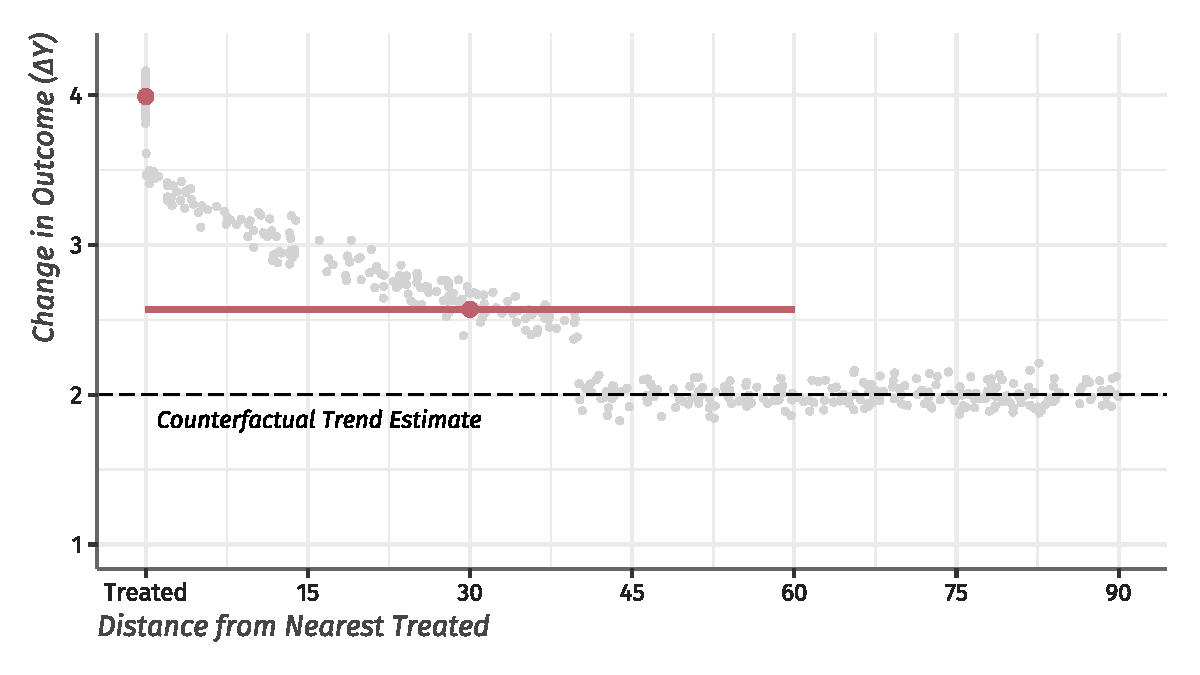
\includegraphics{../../figures/figure-within_example.pdf}
%             }
%         \end{center}
%     \end{figure}
% \end{frame}

% \begin{frame}
%     \begin{figure}[tb!]
%         \caption{Multiple Rings - Improves estimation of spillover effects}
%         \begin{center}
%             \resizebox{0.9\textwidth}{!}{
%                 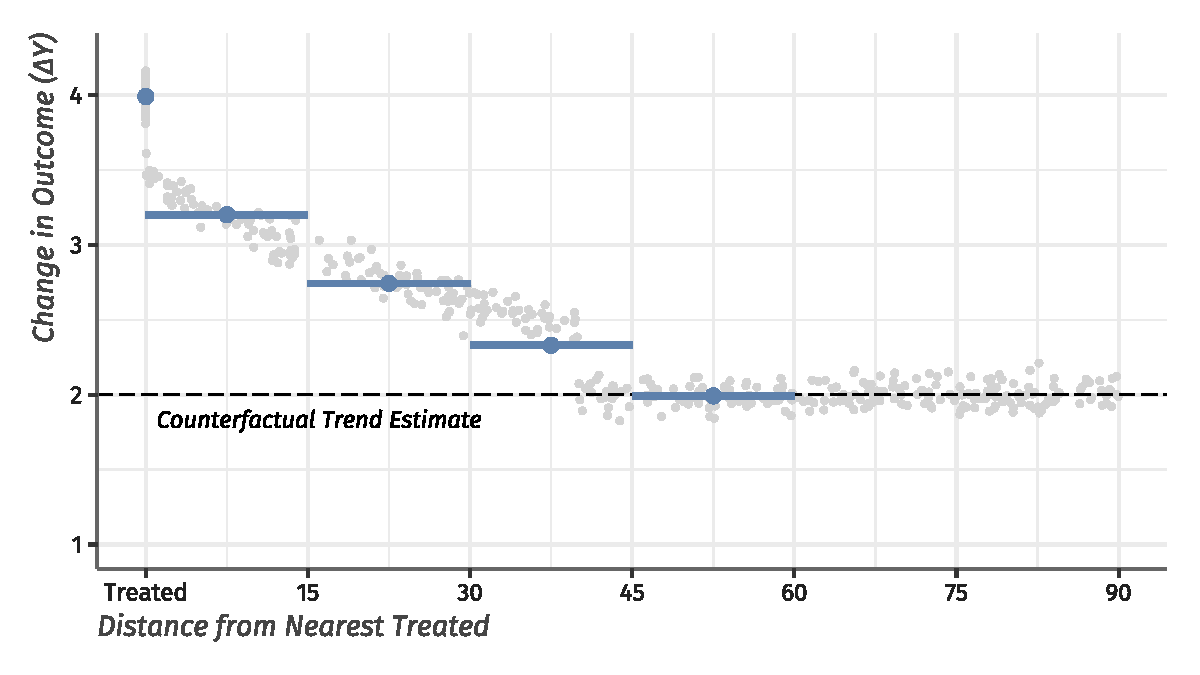
\includegraphics{../../figures/figure-rings_example.pdf}
%                 } 
%             \end{center}
%     \end{figure}
% \end{frame}

% \begin{frame}
%     \begin{figure}[tb!]
%         \caption{Community Health Centers}
%         \begin{center}
%             \resizebox{0.9\textwidth}{!}{
%                 \includegraphics{../../figures/figure-chc-es_combined_slides.pdf}
%                 } 
%             \end{center}
%     \end{figure}
% \end{frame}


% Grey out overlays
\setbeamercovered{transparent}

\begin{frame}{Outline}

    \begin{itemize}
        \item[1--] Formalize spillovers into a potential outcomes framework:
 
        \begin{citecolor}
            [\citet{Clarke_2017}, \citet{Berg_Streitz_2019}, and \citet{Verbitsky-Savitz_Raudenbush_2012}]
        \end{citecolor}

        \begin{itemize}
            \vspace{2.5mm}
            \item I decompose the difference-in-differences estimator into three parts: Direct Effect of Treatment, Spillover onto Treated Units, Spillover onto Control Units
            
            \vspace{2.5mm}
            \item Discuss estimands of interest and classify which are identifiable and which are not
        \end{itemize} 

    \end{itemize}
\end{frame}

\begin{frame}{Outline}
    \begin{itemize}
        \item[2--] Apply framework to Urban Economics
        \begin{itemize}
            \item Revisit \begin{citecolor}\citet{Kline_Moretti_2014a}\end{citecolor} analysis of the Tennessee Valley Authority
            
            \begin{itemize}
                \vspace{2.5mm}
                \item The local effect estimate is contaminated by spillover effects to neighboring counties \begin{citecolor}\citep{Kline_Moretti_2014b}\end{citecolor}
                
                \vspace{2.5mm}
                \item Large scale manufacturing investment creates an `urban shadow' \begin{citecolor}\citep{Cuberes_Desmet_Rappaport_2021,Fujita_Krugman_Venables_2001}\end{citecolor}
            \end{itemize}
            
            \vspace{2.5mm}
            \item Discuss how framework can reconcile conflicting findings on effect of federal Empowerment Zones \begin{citecolor}\citep{Busso_Gregory_Kline_2013,Neumark_Kolko_2010}\end{citecolor}
            
            \vspace{2.5mm}
            \item Event Study estimates of Community Health Centers find highly localized efffects \begin{citecolor}\citep{Bailey_Goodman_Bacon_2015}\end{citecolor}
        \end{itemize}
    \end{itemize} 
\end{frame}



% ------------------------------------------------------------------------------
\section{Theory}
% ------------------------------------------------------------------------------


\begin{frame}{Potential Outcomes Framework}
    For exposition, I will label units as counties. Assume all treatment occurs at the same time (2-periods or pre-post averages).\footnote{I extend this into an event study framework in the paper, but the intuition is the same as in the $2 \times 2$ setting.}
    
    \begin{itemize}
        \item $Y_{it}(D_i, \textcolor{alice}{h(\vec{D}, i)})$ is the potential outcome of county $i \in \{ 1, \dots, N \}$ at time $t$ with treatment status $D_i \in \{0, 1\}$.
        
        \item $\vec{D} \in \{0,1\}^N$ is the vector of all units treatments.
        
        \pause
        \item The function $\textcolor{alice}{h(\vec{D}, i)}$ maps the entire treatment vector into an `exposure mapping' which can be a scalar or a vector.
        
        \pause
        \item No exposure is when $\textcolor{alice}{h(\vec{D}, i)} = \vec{0}$.
    \end{itemize}
\end{frame}

% Grey out
% \setbeamercovered{transparent}

\begin{frame}{Examples of $h_i(\vec{D})$}
    
    Examples of $h_i(\vec{D})$:
    
    \begin{itemize}
        \item \textbf{Treatment within $x$ miles:}
        
        $\textcolor{alice}{h(\vec{D}, i)} = max_j \ 1\left(d(i, j\right) \leq x)$ where $d(i,j)$ is the distance between counties $i$ and $j$. 

        \begin{itemize}
            \item e.g. library access where $x$ is the maximum distance people will travel
            
            \item Spillovers are non-additive, i.e. spillover effects do not depend on number of nearby treated areas
        \end{itemize}

    \end{itemize}
\end{frame}

\begin{frame}{Examples of $h_i(\vec{D})$}
    
    Examples of $h_i(\vec{D})$:
    
    \begin{itemize}
        \item \textbf{Treatment within $x$ miles:}
        
        $\textcolor{alice}{h(\vec{D}, i)} = max_j \ 1(d(i, j) \leq x)$ where $d(i,j)$ is the distance between counties $i$ and $j$. 

        \begin{itemize}
            \item e.g. library access where $x$ is the maximum distance people will travel
            
            \item Spillovers are non-additive
        \end{itemize}
        
        \vspace{2.5mm}
        \item \textbf{Number of Treated within $x$ miles:}
        
        $\textcolor{alice}{h(\vec{D}, i)} = \sum_{j = 1}^k 1(d(i, j) \leq x)$. 

        \begin{itemize}
            \item e.g. Amazon shipping center
            
            \item Agglomeration economies suggest spillovers are additive
        \end{itemize}

    \end{itemize}
\end{frame}

\begin{frame}{Estimands}{Treatment Effect without Spillovers}
    \[
        \tau \equiv \mathbb{E} \left[ Y_i(1) - Y_i(0) \mid D_i = 1\right]
    \]
    \vspace{5mm}

    \begin{itemize}
        \item The average effect of switching on unit $i$'s treatment
    \end{itemize}

    \vspace{60mm}
\end{frame}

\begin{frame}{Estimands}{Switching Effect}
    \[
        \textcolor{maroon}{\tau_{\text{switch}}(h)} \equiv \mathbb{E} \left[ Y_{i1}(1, h_i(\vec{D})) - Y_{i1}(0, h_i(\vec{D})) \mid D_i = 1, h_i(\vec{D}) = h \right]
    \]

    \vspace{5mm}

    \begin{itemize}
        \item Keep everyone's treatment constant and toggle unit $i$'s treatment effect. Average across all units with exposure $h$.
        
        \item This is policy relevant: what will happen if my county turns on treatment.
        \pause

        \item This requires knowledge of $h_i(\vec{D})$ in order to find control units to estimate $Y_{i1}(0, h_i(\vec{D}))$.
    \end{itemize}

    \vspace{60mm}
\end{frame}

\begin{frame}{Estimands}{Switching Effect}
    \begin{align*}
        \textcolor{maroon}{\tau_{\text{switch}}(h)} &= \mathbb{E} \left[ Y_{i1}(1, h_i(\vec{D})) - Y_{i0}(0,\vec{0}) \mid D_i = 1, h_i(\vec{D}) = h \right]\\ 
        &\quad\quad - \textcolor{asher}{\mathbb{E} \left[ Y_{i1}(0, h_i(\vec{D})) - Y_{i0}(0,\vec{0}) \mid D_i = 1, h_i(\vec{D}) = h \right]} 
    \end{align*}
        
    \vspace{5mm}
    Identification requires two things:
    \begin{enumerate}
        \item Knowledge of $h_i(\vec{D})$ in order to estimate the second term with control units.
        
        \item Spillover effect homogeneity (so second term would be the same for treated units).
    \end{enumerate}
    \vspace{60mm}
\end{frame}


\begin{frame}{Estimands}{Total Effect}
    \[
        \textcolor{navy}{\tau_{\text{total}}} \equiv \mathbb{E} \left[ Y_{i1}(1, h_i(\vec{D})) - Y_{i1}(0, \vec{0}) \mid D_i = 1 \right]
    \]

    \vspace{5mm}
    \begin{itemize}
        \item Toggle entire vector of treatment effects. Average across all treated units.
        
        \item This is helpful for post-hoc policy analysis: what was the average effect on treated units of implementing $\vec{D}$.
    \end{itemize}

    \vspace{60mm}
\end{frame}

\begin{frame}{Estimands}{Total Effect}
    \begin{align*}
        \textcolor{navy}{\tau_{\text{total}}} &= \mathbb{E} \left[ Y_{i1}(1, h_i(\vec{D})) - Y_{i0}(0,\vec{0}) \mid D_i = 1\right]\\ 
        &\quad\quad - \textcolor{asher}{\mathbb{E} \left[ Y_{i1}(0, \vec{0}) - Y_{i0}(0,\vec{0}) \mid D_i = 1 \right]} 
    \end{align*}
        
    \vspace{5mm}
    Identification much simpler:
    \begin{itemize}
        \item Need to identify control units without spillover effects
    \end{itemize}
    \vspace{60mm}
\end{frame}

\begin{frame}{Estimands}{Direct Effect}
    \[
        \textcolor{kelly}{\tau_{\text{direct}}} \equiv \mathbb{E} \left[ Y_{i1}(1, \vec{0}) - Y_{i1}(0, \vec{0}) \mid D_i = 1 \right]
    \]

    \vspace{5mm}
    \begin{itemize}
        \item Toggle treatment effect for individuals with no exposure.
        
        \item This is the switching effect with $h = 0$.
        
        \pause
        \item Identified under mild assumptions.
    \end{itemize}

    \vspace{60mm}
\end{frame}

\begin{frame}{Estimands}{Direct Effect}
    \begin{align*}
        \textcolor{kelly}{\tau_{\text{direct}}} &= \mathbb{E} \left[ Y_{i1}(1, \vec{0}) - Y_{i0}(0,\vec{0}) \mid D_i = 1 \right]\\ 
        &\quad\quad - \textcolor{asher}{\mathbb{E} \left[ Y_{i1}(0, \vec{0}) - Y_{i0}(0,\vec{0}) \mid D_i = 1 \right]} 
    \end{align*}
        
    \vspace{5mm}
    Identification much simpler:
    \begin{itemize}
        \item Need to identify treated/control units without spillover effects
    \end{itemize}
    \vspace{60mm}
\end{frame}


\begin{frame}{Estimands}{Spillover Effects}
    \[
        \textcolor{red}{\tau_{\text{spillover, treated}}} \equiv \mathbb{E} \left[ Y_{i1}(1, h_i(\vec{D})) - Y_{i1}(1, 0) \mid D_i = 1 \right]
    \]

    \[ 
        \textcolor{coral}{\tau_{\text{spillover, control}}} \equiv \mathbb{E} \left[ Y_{i1}(0, h_i(\vec{D})) - Y_{i1}(0, 0) \mid D_i = 0 \right]
    \]
    \vspace{5mm}
    \vspace{60mm}
\end{frame}


\begin{frame}{What does Difference-in-Differences identify?}{Parallel Trends}
    I assume a modified version of the parallel counterfactual trends assumption: 

    \vspace{2.5mm}
    \begin{block}{Assumption: {\it Parallel Counterfactual Trends}}
        \vspace{-5mm}
        \begin{align*}
            \mathbb{E}\big[ \underbrace{Y_{i,1}(0, \textcolor{alice}{\vec{0}}) - Y_{i,0}(0, \textcolor{alice}{\vec{0}})}_{\text{Counterfactual Trend}} \mid D_i = 1 \big] = \ \mathbb{E}\big[ \underbrace{Y_{i,1}(0, \textcolor{alice}{\vec{0}}) - Y_{i,0}(0, \textcolor{alice}{\vec{0}})}_{\text{Counterfactual Trend}} \mid D_i = 0 \big]
        \end{align*}
    \end{block}

    In the \emph{complete absence of treatment} (not just the absence of individual $i$'s treatment):
    
    Changes in outcomes do not depend on treatment status
    
\end{frame}

\begin{frame}{What does Difference-in-Differences identify?}{Decomposition}
    With the parallel trends assumption, I decompose the difference-in-differences estimate as follows: 
        
    \begin{align*}
        \mathbb{E}\left[\hat{\tau}\right] &= \underbrace{\mathbb{E} \left[ Y_{i1} - Y_{i0} \mid D_i = 1 \right] - \mathbb{E} \left[ Y_{i1} - Y_{i0} \mid D_i = 0 \right]}_{\text{Difference-in-Differences}} \\[3mm]
        \pause&= \tau_{\text{direct}} + \textcolor{red}{\tau_{\text{spillover, treated}}} - \textcolor{coral}{\tau_{\text{spillover, control}}} \\[3mm]
        \pause&= \tau_{\text{total}} - \textcolor{coral}{\tau_{\text{spillover, control}}} 
    \end{align*}

\end{frame}


\begin{frame}{Identification of Direct/Total Effects}
    \begin{block}{Assumption: {\it Spillovers are Local}}

    Let $d(i,j)$ be the distance between units $i$ and $j$. There exists a distance $\bar{d}$ such that 
        
        (i) For all units $i$,
        \[ 
            \min_{j: D_j = 1} d(i,j) > \bar{d} \implies h(\vec{D}, i) = \vec{0}. 
        \]
    
        (ii) There are treated and control units such that $\min_{j: \ D_j = 1} d(i,j) > \bar{d}$.

    \end{block}
\end{frame}


\begin{frame}{Identification of Total Effect}
    With assumption that spillovers are local, define $S_{it}$ to be an indicator equal to one in the post period for all units with $h(\vec{D}, i) \neq \vec{0}$ (and potentially some units with $= \vec{0}$).

    \vspace{5mm}
    Estimation of the following equation:
    \[ 
        y_{it} = \mu_t + \mu_i + \tau D_{it} + \tau_{\text{spill,control}} S_{it} * (1-D_{it}) + \varepsilon_{it}
    \]

    \begin{itemize}
        \item $\hat{\tau}$ is consistent for $\tau_{\text{total}}$
        
        \item $\hat{\tau}_{\text{spill, control}}$ is not consistent for average spillover effects. 
    \end{itemize}
\end{frame}

\begin{frame}{Identification of Direct Effect}
    With assumption that spillovers are local, define $S_{it}$ to be an indicator equal to one in the post period for all units with $h(\vec{D}, i) \neq \vec{0}$ (and potentially some units with $= \vec{0}$).

    \vspace{5mm}
    Estimation of the following equation:
    \[ 
        y_{it} = \mu_t + \mu_i + \tau D_{it} + \tau_{\text{spill,treat}} S_{it} * D_{it} + \tau_{\text{spill,control}} S_{it} * (1-D_{it}) + \varepsilon_{it}
    \]

    \begin{itemize}
        \item $\hat{\tau}$ is consistent for $\tau_{\text{direct}}$
        
        \item $\hat{\tau}_{\text{spill}}$'s are not consistent for average spillover effects.
    \end{itemize}

\end{frame}

% ------------------------------------------------------------------------------
\section{Application in Urban Economics}
% ------------------------------------------------------------------------------

\begin{frame}{Tennessee Valley Authority}
    \citet{Kline_Moretti_2014a} look at the long-run impacts of the Tennessee Valley Authority (TVA).

    \begin{itemize}
        \item The TVA was a large-scale federal investment started in 1934 that focused on improving manufacturing economy. (Hundreds of dollars spent anually per person)
        
        \item The program focused on large-scale dam construction that brought cheap wholesale electricity to the region
    \end{itemize}

    \pause
    Research Questions:
    \begin{itemize}
        \item What is the total effect of TVA investments on manufacturing and agricultural employment?
        \item Do these effects come at the cost of other counties?
    \end{itemize}
\end{frame}

\begin{frame}{Identification}
    \citet{Kline_Moretti_2014a} run the county-level difference-in-differences  specification: 
    \begin{equation}\label{eq:tva_spillover}
        y_{c, 2000} - y_{c, 1940} = \alpha + \text{TVA}_c \tau + X_{c, 1940} \beta + (\varepsilon_{c, 2000} - \varepsilon_{c, 1940})
    \end{equation} 

    \begin{itemize}
        \item $y$ are outcomes for agricultural employment and manufacturing employment.
        \item $\text{TVA}_c$ is the treatment variable
        \item $X_{c, 1940}$ allow for different long-term trends based on covariates in 1940. 
    \end{itemize}

    They trim the sample using a logit regression to predict treatment using $X_{c,1940}$ and then keep control units in the top 75\% of predicted probability.
\end{frame}

\begin{frame}{Spillovers in the TVA Context}
    In our context, there is reason to believe spillovers can occur to nearby counties

    \begin{itemize}
        \item \textbf{Agriculture:} 
        \begin{itemize}
            \item Employees might be drawn to hire wages for new manufacturing jobs in Tennessee Valley (negative spillover on control units)
        \end{itemize}
        
        \item \textbf{Manufacturing:}
        \begin{itemize}
            \item Cheap electricity might be available to nearby counties (positive spillover on control units) 
            
            \item Manufacturing jobs that would have been created in the control units in the absence of treatment might move to the Tennessee Valley (negative spillover on control units)
        \end{itemize}
    \end{itemize}
\end{frame}

\begin{frame}{Specification including spillovers}
    \begin{equation}
        \Delta y_c = \alpha + \text{TVA}_i \tau + \sum_{d \in \text{Dist}} \text{Ring}(d)\delta_d + X_{i, 1940} \beta + \Delta \varepsilon_c
    \end{equation} 

    \begin{itemize}
        \item $\text{Ring}(d)$ is a set of indicators for being in the following distance bins (in miles) from the Tennessee Valley Authority: 
        \[ d \in \left\{ (0, 50], (50, 100], (100, 150] (150, 200]\right\} \]
    \end{itemize}
\end{frame}

\imageframe{../../figures/figure-tva-sample_slides.pdf}

\begin{frame}
\begin{table}[ht]
    \caption{Effects of Tennessee Valley Authority on Decadel Growth, 1940-2000}
    \label{tab:tva}
    \renewcommand{\arraystretch}{1.2}

    \begin{adjustbox}{width = 1\textwidth, center}
        \begin{threeparttable}
            \begin{tabular}{@{} l c@{\extracolsep{20pt}}c@{\extracolsep{4pt}}cccc @{}}
                % Head
                \toprule

                & \multicolumn{1}{c}{\textbf{Diff-in-Diff}} & \multicolumn{5}{c}{\textbf{Diff-in-Diff with Spillovers}} \\ 
                \cmidrule{2-2} \cmidrule{3-7}
                & & & TVA between & TVA between & TVA between & TVA between \\ 
                & TVA & TVA & 0-50 mi. & 50-100 mi. & 100-150 mi. & 150-200 mi. \\ 
                \textit{Dependent Var.} & (1) & (2) & (3) & (4) & (5) & (6) \\

                % Body
                \midrule
                
                Agricultural employment     & $-0.0514^{***}$ & $-0.0739^{***}$& $-0.0371^{***}$&    $-0.0164$   & $-0.0298^{***}$&  $-0.0157^{*}$ \\
                &   $(0.0114)$   &   $(0.0142)$   &   $(0.0002)$   &   $(0.0114)$   &   $(0.0096)$   &   $(0.0088)$

                \onslide<2->{
                    \\
                    Manufacturing employment    & $0.0560^{***}$ &    $0.0350$    & $-0.0203^{***}$&    $-0.0245$   &  $-0.0331^{*}$ & $-0.0296^{**}$ \\
                    &   $(0.0161)$   &   $(0.0218)$   &   $(0.0006)$   &   $(0.0282)$   &   $(0.0189)$   &   $(0.0142)$ 
                }
               
                \\ \bottomrule
            \end{tabular}
            
            % Notes 
            \begin{tablenotes}\footnotesize

                \item $^{*} p< 0.1$; $^{**} p < 0.05$; $^{***} p < 0.01$.
            \end{tablenotes}
        \end{threeparttable}
    \end{adjustbox}
\end{table}    

\end{frame}


\begin{frame}{Identification Strategies and Place-Based Policies}

    The literature on federal Enterprise Zones, place-based policy that gives tax breaks to businesses that locate within the boundary, has found conflicting results, suggesting positive or near-zero effects of the program \citep{Neumark_Young_2019}. 


\end{frame}

\begin{frame}{Identification Strategies and Place-Based Policies}
    
    \begin{itemize}
        \item \citet{Busso_Gregory_Kline_2013} compare census tracts in Empowerment Zones to census tracts that qualified and were rejected from the program. They find significant large reduction of poverty.
        
        \pause
        \item \citet{Neumark_Kolko_2010} compare census tracts in Empowerment Zones to census tracts within 1,000 feet of the Zone. They find near-zero effects on poverty.
    \end{itemize}

    \pause
    My framework can explain both of these results. If census tracts just outside the Empowerment Zones also benefit from the policy, then the estimates of \citet{Neumark_Kolko_2010} are attenuated towards zero

\end{frame}

\section{Event Study}

\begin{frame}{Gardner (2021) Overview}

    \[ 
        y_{it} = \mu_i + \mu_t + \tau D_{it} + \varepsilon_{it}
    \]

    The problem with estimating this by OLS is that the treatment variable becomes residualized $\tilde{D}_{it}$ and this leads to all sorts of problems... (see new diff-in-diff literature)

    \pause

    Gardner (2021) recommends a two-step approach:

    1. Estimate $\mu_i$ and $\mu_t$ using never-treated/not-year-treated observations ($D_{it}$ = 0). Then subtract off $\hat{\mu}_i$ and $\hat{\mu}_t$.
        
    \pause
    2. Then, regress $y_{it} - \hat{\mu}_i - \hat{\mu}_t \equiv \tilde{y}_{it}$ on $\tau D_{it}$ (or event study leads/lags). This estimate is unbiased because $D_{it}$ is non-residualized (standard errors require adjusting).
\end{frame}

\begin{frame}{Controlling for Spillovers in Staggered Treatment Timing}
    \[ 
        y_{it} = \mu_i + \mu_t + \tau D_{it} + {\color{coral} \tau_{\text{spill,control}} S_{it} * (1-D_{it}) } + {\color{kelly} \tau_{\text{spill,treat}} S_{it} * D_{it}} + \varepsilon_{it}
    \]

    Adjust two-step approach:

    \pause

    1. Estimate $\mu_i$ and $\mu_t$ using observations that are not yet treated/affected by spillovers ($D_{it} = 0$ and $S_{it} = 0$). Then subtract off $\hat{\mu}_i$ and $\hat{\mu}_t$.  
    
    2. Then, regress $\tilde{y}_{it}$ on $\tau D_{it} + {\color{coral} \tau_{\text{spill,control}} S_{it} * (1-D_{it}) } + {\color{kelly} \tau_{\text{spill,treat}} S_{it} * D_{it}}$ (or interacted event study leads/lags). This estimate is unbiased because $D_{it}$ is non-residualized (standard errors require adjusting).

\end{frame}

\begin{frame}{Community Health Centers}
    \begin{citecolor}\citet{Bailey_Goodman_Bacon_2015}\end{citecolor} study the creation of federal community health centers between 1965 and 1974.
    
    \vspace{5mm}
    Research Question:
    
    \begin{itemize}
        \item Do low-/no-cost health services lower the mortality rate of the treated counties? 
        \item \emph{New Question:} Do these effects spread to neighboring counties?
    \end{itemize}
\end{frame}

\begin{frame}
    \begin{figure}[tb!]
        \caption{Effects of Establishment of Community Health Centers}
        \begin{center}
            \resizebox{0.9\textwidth}{!}{
                \includegraphics[width=\textwidth]{../../figures/figure-chc-es_original.pdf}
            }
        \end{center}
    \end{figure}
\end{frame}

\begin{frame}
    \begin{figure}[tb!]
        \caption{Direct and Spillover Effects of Community Health Centers}
        \begin{center}
            \resizebox{0.9\textwidth}{!}{
                \includegraphics[width=\textwidth]{../../figures/figure-chc-es_combined.pdf}
            }
        \end{center}
    \end{figure}
\end{frame}

\section{Conclusion}

\begin{frame}{Conclusion}
    \begin{itemize}
        \item I decomposed the TWFE estimate into the direct effect and two spillover terms
        
        \item I showed that a set of concentric rings allows for estimation of the direct effect of treatment and they are able to model spillovers well
        
        \item For place-based policies, I show the importance of considering spatial spillovers when estimating treatment effects
        
        \item More generally, identification strategies that use very close control units in order to minimize differences in unobservables should consider the problems with treatment effect spillovers.
    \end{itemize}
\end{frame}





















\end{document}
